\documentclass{standalone}
\usepackage{tikz}
\usetikzlibrary{arrows.meta}
\tikzset{label/.style = {inner sep=1pt, fill=white}}
%\tikzset{nd/.style={circle, inner sep=0pt}}
\tikzset{nd/.style={inner sep=1pt}}
\tikzset{>=Latex}
\tikzset{arc/.style = {->, semithick, >=Latex}}
\begin{document}
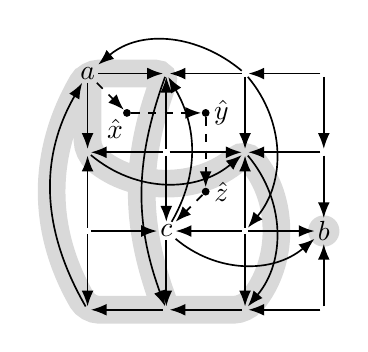
\begin{tikzpicture}

\draw [rounded corners, color = gray!30, line width = 10pt] (1,2) to [in = 110, out = -110] (1,-1) -- (0,-1) to [in = -120, out = 120] (0,2) -- (0,1) to[in = 220, out = -40] (2,1) to [in = 50, out = -50] (2,-1) -- (1,-1) -- (0,-1) to [in = -120, out = 120] (0,2) -- cycle;

\node[nd,color = gray!30, circle, inner sep= 4pt, fill] at (3,0) {};

    \node[nd] (1) at (0,0) {};
    \node[nd] (2) at (1,0) {$c$};
    \node[nd] (3) at (2,0) {};
    \node[nd] (4) at (0,1) {};
    \node[nd] (5) at (1,1) {};
    \node[nd] (6) at (2,1) {};
    \node[nd] (7) at (0,2) {$a$};
    \node[nd] (8) at (1,2) {};
    \node[nd] (9) at (2,2) {};

    \node[nd] (10) at (0,-1) {};
    \node[nd] (11) at (1,-1) {};
    \node[nd] (12) at (2,-1) {};
    %\node[nd] (13) at (3,-1) {13};

    \node[nd] (14) at (3,0) {$b$};
    \node[nd] (15) at (3,-1) {};
    \node[nd] (16) at (3,1) {};
    \node[nd] (17) at (3,2) {};

    \draw[arc] (3) to (14);
    \draw[arc] (2) to[out = -40, in = -140] (14);
    \draw[arc] (1) to (2);
    \draw[arc] (1) to (4);
    \draw[arc] (1) to (10);
    \draw[arc] (17) to (16);
    \draw[arc] (16) to (14);
    \draw[arc] (15) to (14);
    \draw[arc] (15) to (12);
    \draw[arc] (12) to (11);
    \draw[arc] (11) to (10);
    \draw[arc] (10) to [in = -120, out = 120] (7);
    \draw[arc] (17) to (9);
    \draw[arc] (16) to (6);
    \draw[arc] (6) to [in = 50, out = -50] (12);
    \draw[arc] (3) to (12);
    \draw[arc] (8) to [in = 110, out = -110] (11);
    \draw[arc] (2) to (11);
    
    %\draw[arc] (4) to (1);
    %\draw[arc] (3) to[in = -40, out = 220] (1);
    \draw[arc] (9) to[in = 50, out = -50] (3);
    \draw[arc] (9) to (8);
    \draw[arc] (5) to (8);
    \draw[arc] (5) to (4);
    
    \draw[arc] (7) to (4);
    %\draw[arc] (7) to[in = 130, out = -130] (1);
    \draw[arc] (7) to (8);
    \draw[arc] (9) to[out = 140, in = 40] (7);
    %\draw[arc] (1) to (2);
    \draw[arc] (3) to (2);
    \draw[arc] (5) to (2);
    \draw[arc] (2) to[in = -60, out = 60] (8);
    \draw[arc] (3) to (6);
    \draw[arc] (9) to (6);
    \draw[arc] (5) to (6);
    \draw[arc] (4) to[in = 220, out = -40] (6);

    \node[nd, circle, inner sep= 1pt, fill] (x) at (0.5,1.5) {};
    \node at (0.35,1.3) {$\hat x$};

    \node[nd, circle, inner sep= 1pt, fill] (y) at (1.5,1.5) {};
    \node at (1.7,1.5) {$\hat y$};

    \node[nd, circle, inner sep= 1pt, fill] (z) at (1.5,0.5) {};
    \node at (1.7,0.5) {$\hat z$};

    \draw[arc,dashed] (7) to (x);
    \draw[arc,dashed] (x) to (y);
    \draw[arc,dashed] (y) to (z);
    \draw[arc,dashed] (z) to (2);
    
 \end{tikzpicture}
\end{document}